\section{Frontend}

\subsection{Descrizione generale}

Il frontend dell'applicazione andrà a costituire il ruolo di \textit{View} nel pattern MVC. In particolare tale componente dell'applicazione è costituita da un sottosistema che implementa l'architettura \textit{Flux} proposta da \textit{Facebook}. Tale architettura si basa sul creare un sistema che abbia un \textit{data-flow} unidirezionale al fine di semplificare le interazioni tra le varie componenti e di assicurare che tra le componenti non esistano dipendenze circolari.
Nella progettazione secondo l'architettura \textit{Flux} si è seguito in particolare il principio che nessuna classe modifichi direttamente lo stato di un'altra ma che vengano create delle componenti che richiedono un'interazione delle \textit{Action} per comunicare con le altre parti del sistema.

\begin{figure}[h]
\centering
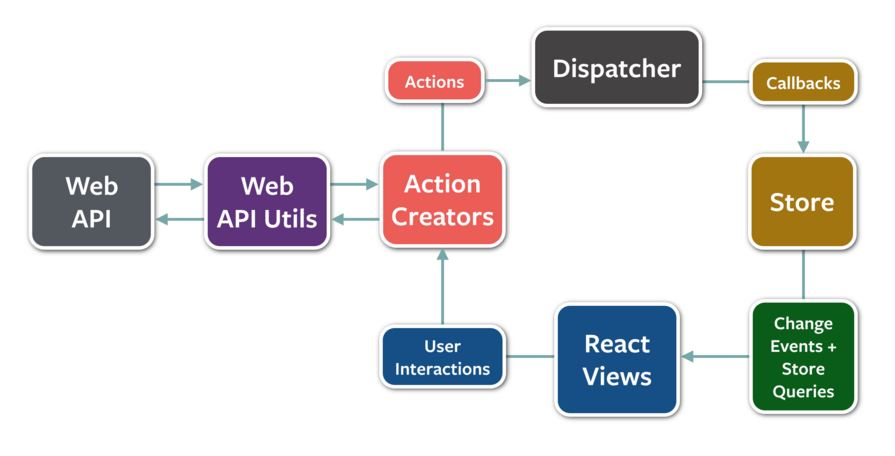
\includegraphics[width=0.8\textwidth]{res/sections/imgs/flux.jpg}
\caption{Diagramma dell'architettura Flux di Facebook}
\end{figure}
In un'architettura \textit{Flux} vengono distinti 4 componenti fondamentali:

\begin{itemize}
\item \textbf{Action}: Rappresenta un messaggio tra le componenti del sistema;
\item \textbf{Dispatcher}: funge da \textit{hub} centrale per le \textit{action} e si occupa di distribuirle al giusto \textit{store};
\item \textbf{Store}: contengono la logica applicativa del frontend e lo stato dei dati dall'ultimo \textit{update}. Si occupano di fornire i dati alle viste, quando queste li richiedono;
\item \textbf{View}: Sono la parte visiva dell'applicazione e, nel nostro caso, saranno costituite da componenti definite con React.
\end{itemize}

Dall'architettura sopra descritta sono stati individuati i seguenti \glossaryItem{package} per il lato frontend di \glossaryItem{MaaS}:

\begin{figure}[H]
\centering
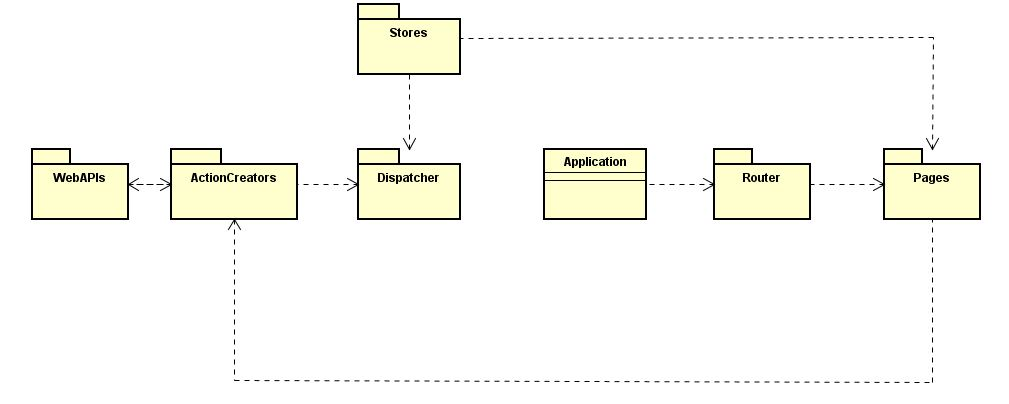
\includegraphics[width=0.8\textwidth]{res/sections/imgs/packages-diagram.jpg}
\caption{Diagramma dei \glossaryItem{package} del frontend}
\end{figure}

\begin{figure}[H]
\centering
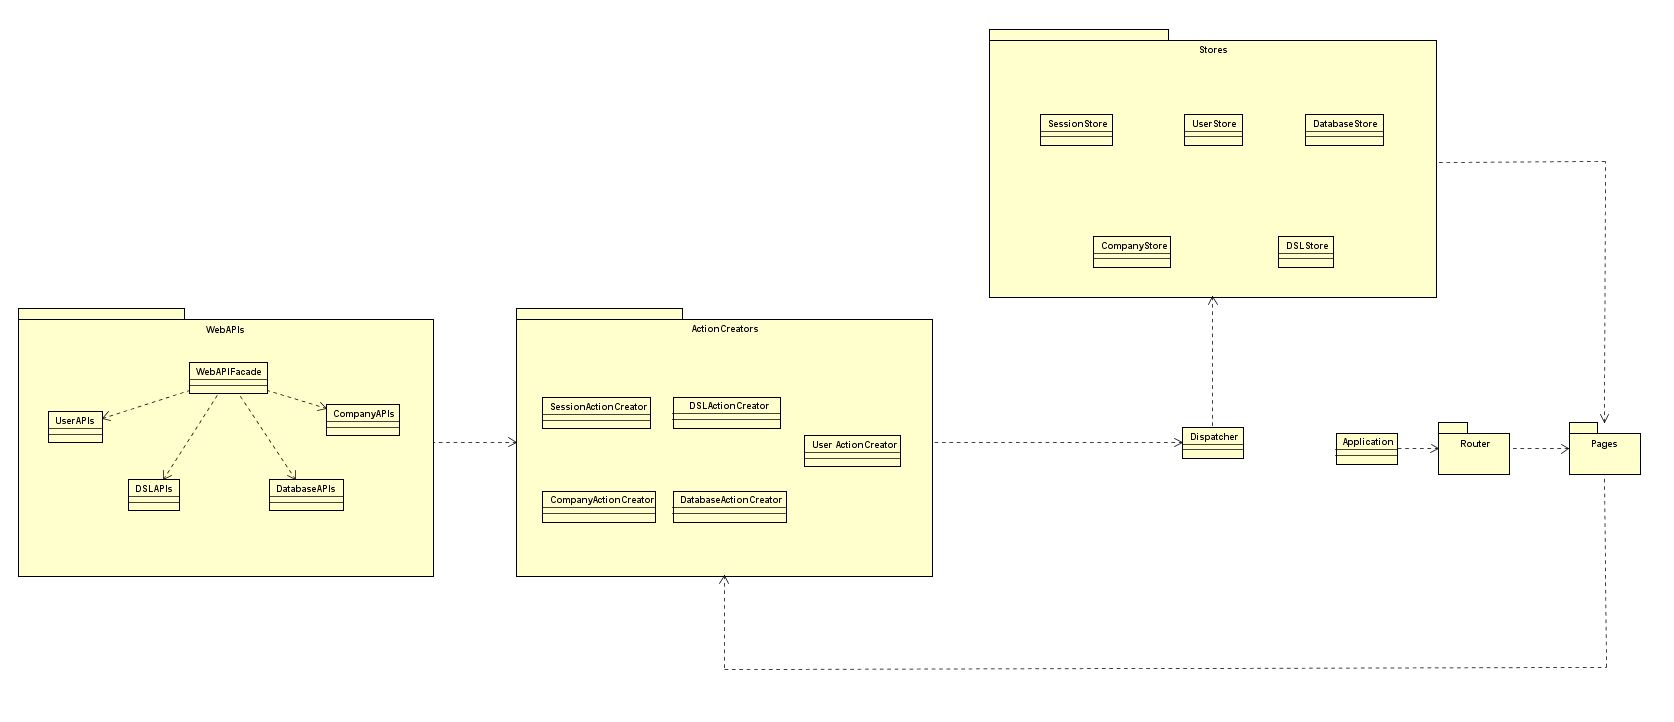
\includegraphics[width=0.8\textwidth]{res/sections/frontend/fullFrontend.jpg}
\caption{Diagramma delle classi del Frontend}
\end{figure}

\subsection{WebAPIs}

\begin{figure}[h]
\centering
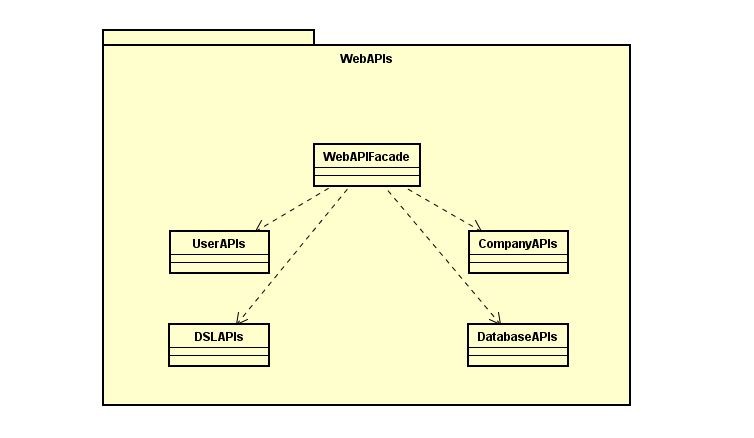
\includegraphics[width=0.8\textwidth]{res/sections/imgs/webapi-diagram.jpg}
\caption{Diagramma del \glossaryItem{package} webAPIs}
\end{figure}

\paragraph*{Descrizione del \glossaryItem{package}}
Il seguente \glossaryItem{package} contiene tutte le classi che contengono i metodi per interagire con le \glossaryItem{API} esposte dal server. 
\paragraph*{Classi contenute}
\begin{itemize}
\item \textbf{UserAPIs};
\item \textbf{CompanyAPIs};
\item \textbf{DSLAPIs};
\item \textbf{DatabaseAPIs};
\item \textbf{WebAPIFacade}.
\end{itemize}

\subsubsection{UserAPIs}
\paragraph*{Descrizione della classe}
Classe che espone tutti i metodi per interagire con le \glossaryItem{API} del server che riguardano gli utenti.

\paragraph*{Utilizzo}
Viene utilizzata sia per il login sia per gestire le operazioni CRUD per le informazioni riguardanti gli utenti.

\paragraph*{Relazione con altre classi}
\begin{itemize}
\item ActionCreators::UserActionCreator. La classe UserAPIs fornisce i metodi affichè UserActionCreator possa interagire con il server.
\end{itemize}

\subsubsection{CompanyAPIs}
\paragraph*{Descrizione della classe}
Classe che espone i metodi per interagire con le \glossaryItem{API} esposte dal server che riguardano le \glossaryItem{Company}.

\paragraph*{Utilizzo}
Contiene le operazioni CRUD per interagire con le informazioni riguardanti le \glossaryItem{company} utilizzando le \glossaryItem{API} esposte dal backend.

\paragraph*{Relazione con altre classi}
\begin{itemize}
\item ActionCreators::CompanyActionCreator. La classe CompanyAPIs fornisce i metodi affinchè CompanyActionCreator possa interagire con le \glossaryItem{API} riguardanti le \glossaryItem{Company} fornite dal backend.
\end{itemize}

\subsubsection{DSLAPIs}
\paragraph*{Descrizione della classe}
Classe che espone i metodi per interagire con le \glossaryItem{API} esposte dal server che riguardano le specifiche \glossaryItem{DSL}.

\paragraph*{Utilizzo}
Viene utilizzata per lanciare le operazioni CRUD associate alle \glossaryItem{API} esposte dal backend.

\paragraph*{Relazione con altre classi}
\begin{itemize}
\item ActionCreators::DSLActionCreator. La classe DSLAPIs fornisce i metodi affinchè DSLActionCreator possa interagire con le \glossaryItem{API} righardanti le specifiche \glossaryItem{DSL} fornite dal backend.
\end{itemize}

\subsubsection{DatabaseAPIs}
\paragraph*{Descrizione della classe}
Classe per interagire con le \glossaryItem{API} esposte dal server che riguardano i database delle \glossaryItem{Company}.

\paragraph*{Utilizzo}
Viene utilizzata questa classe per lanciare le operazioni CRUD esposte dalle \glossaryItem{API} del backend.

\paragraph*{Relazione con altre classi}
\begin{itemize}
\item ActionCreators::DatabaseActionCreator. La classe DatabaseAPIs fornisce i metodi affinchè DatabaseActionCreator possa interagire con le \glossaryItem{API} riguardanti le connessioni ai database fornite dal server.
\end{itemize}

\subsubsection{WebAPIFacade}
\paragraph*{Descrizione della classe}
Classe che implementa il \textit{design pattern} \textit{Facade} al fine di creare un'interfaccia semplificata per il resto delle componenti per interagire con le \glossaryItem{API} esposte dal backend.
\paragraph*{Utilizzo}
Questa classe viene utilizzata come interfaccia per il frontend per comunicare con le \glossaryItem{API} esposte dal backend.
\paragraph*{Relazione con altre classi}
\begin{itemize}
\item WebAPIs. WebAPIFacade include le altre classi contenute nel \glossaryItem{package} per fornire un interfaccia unica al sistema per comunicare con il backend.
\item ActionCreators. WebAPIFacade è utilizzato dalle classi del \glossaryItem{package} actionCreators per permettere alle classi di quest'ultimo di poter accedere alle \glossaryItem{API} esposte dal server. 
\end{itemize} 

\subsection{ActionCreators}

\begin{figure}[h]
\centering
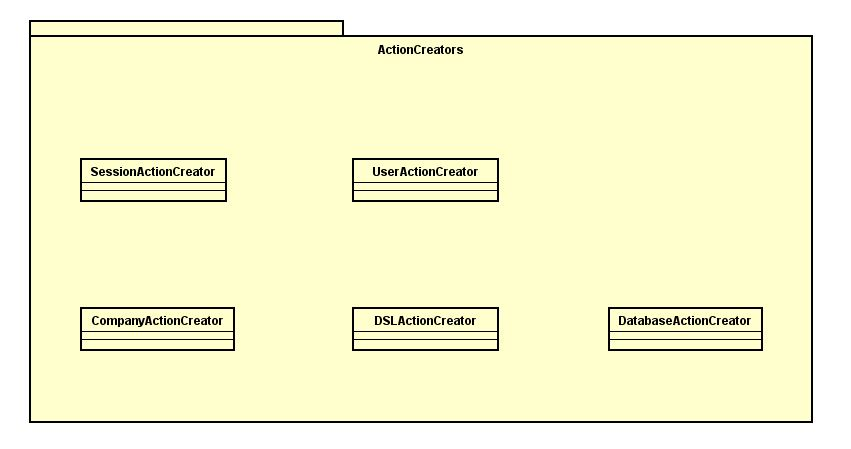
\includegraphics[width=0.8\textwidth]{res/sections/imgs/actioncreator-diagram.jpg}
\caption{Diagramma delle classi contenute in ActionCreators}
\end{figure}

\paragraph*{Descrizione del \glossaryItem{package}}
Questo \glossaryItem{package} contiene tutte le classi che si prestano come factory di \glossaryItem{Action}. Le classi in questione mettono in relazione le webAPIs con il resto dell'applicazione, cioè vengono utilizzate per la richiesta delle funzionalità delle webAPIs per poi lanciare le \glossaryItem{Action} relative alle risposte ricevute.

\paragraph*{Classi contenute}
\begin{itemize}
\item \textbf{SessionActionCreator};
\item \textbf{UserActionCreator};
\item \textbf{CompanyActionCreator};
\item \textbf{DSLActionCreator};
\item \textbf{DatabaseActionCreator}.
\end{itemize}

\subsubsection{SessionActionCreator}
\paragraph*{Descrizione della classe}
Classe che si occupa della gestione delle \textit{action} relative alla sessione corrente.

\paragraph*{Utilizzo}
Viene utilizzata per richiedere il login di un utente e per emanare le \textit{action} relative a login, sessione corrente e logout.

\paragraph*{Relazione con altre classi}
\begin{itemize}
\item Dispatcher: le \glossaryItem{Action} create vengono poi instradate prima al Dispatcher, che poi provvede ad inoltrarle al giusto store.
\item Pages: le pagine definite nel \glossaryItem{package} Pages possono richiamare i metodi di questa classe per effettuare operazioni sulla sessione corrente.
\item WebAPIs::WebAPIFacade: questa classe viene utilizzata per permettere all'ActionCreator di interagire con le \glossaryItem{API} esposte dal backend.
\item Stores::SessionStore: le \glossaryItem{Action} create da SessionActionCreator poi vengono utilizzate da SessionStore per aggiornare lo stato di questi dati nel frontend.
\end{itemize}

\subsubsection{UserActionCreator}
\paragraph*{Descrizione della classe}
Classe che si occupa di creare e lanciare le \textit{action} relative agli utenti. Viene implementata tramite il \textit{design pattern} \textit{Factory}.
\paragraph*{Utilizzo}
Viene utilizzata per creare le \textit{action} relative agli utenti: la classe fornisce i metodi per utilizzare le \textit{webAPIs} contenute relative all'utente e restituisce le \glossaryItem{action} che poi verrano reindirizzate a UserStore.

\paragraph*{Relazione con altre classi}
\begin{itemize}
\item Dispatcher: le \glossaryItem{Action} create vengono poi instradate prima al Dispatcher, che poi provvede ad inoltrarle al giusto store.
\item Pages: le pagine definite nel \glossaryItem{package} Pages possono richiamare i metodi di questa classe per effettuare operazioni sulla gestione degli utenti.
\item webAPIs::WebAPIFacade: questa classe viene utilizzata per permettere all'ActionCreator di interagire con le \glossaryItem{API} esposte dal backend.
\item Stores::UserStore: le \glossaryItem{Action} create da UserActionCreator poi vengono utilizzate da UserStore per aggiornare lo stato dei dati relativi agli utenti nel frontend.
\end{itemize}

\subsubsection{CompanyActionCreator}
\paragraph*{Descrizione della classe}
Classe che si occupa dell'interazione dell'applicazione con CompanyAPIs e di lanciare \textit{Action} relative alle risposte ottenute da essa. Viene implementata tramite \textit{design pattern} \textit{Factory}.
\paragraph*{Utilizzo}
La classe viene utilizzata per creare le \textit{action} relative alle \glossaryItem{Company}: sfrutta le \textit{webAPIs} dichiarate per interagire con il server e lancia le \textit{action} contenenti i dati ricevuti dalle \glossaryItem{API} richieste.

\paragraph*{Relazione con altre classi}
\begin{itemize}
\item Dispatcher: le \glossaryItem{Action} create vengono poi instradate prima al Dispatcher, che poi provvede ad inoltrarle al giusto store.
\item Pages: le pagine definite nel \glossaryItem{package} Pages possono richiamare i metodi di questa classe per effettuare operazioni sulla gestione degli utenti.
\item webAPIs::WebAPIFacade: questa classe viene utilizzata per permettere all'ActionCreator di interagire con le \glossaryItem{API} esposte dal backend.
\item Stores::CompanyStore: le \glossaryItem{Action} create da CompanyActionCreator poi vengono utilizzate da CompanyStore per aggiornare i dati relativi alle \glossaryItem{Company} nel frontend.
\end{itemize}

\subsubsection{DSLActionCreator}
\paragraph*{Descrizione della classe}
Classe che si occupa di creare \textit{action} riguardanti le specifiche \glossaryItem{DSL}.
\paragraph*{Utilizzo}
Tale classe viene utilizzata per sfruttare i metodi dichiarati dalle webAPIs per la richiesta delle \glossaryItem{API} esposte dal server relative alle specifiche \glossaryItem{DSL}. Dopo aver sfruttato l'API richiesta, la classe crea un'\textit{action} contenente i risultati ottenuti.

\paragraph*{Relazione con altre classi}
\begin{itemize}
\item Dispatcher: le \glossaryItem{Action} create vengono poi instradate prima al Dispatcher, che poi provvede ad inoltrarle al giusto store.
\item Pages: le pagine definite nel \glossaryItem{package} Pages possono richiamare i metodi di questa classe per effettuare operazioni sulla gestione degli utenti.
\item webAPIs::WebAPIFacade: questa classe viene utilizzata per permettere all'ActionCreator di interagire con le \glossaryItem{API} esposte dal backend.
\item Stores::DSLStore: le \glossaryItem{Action} create da DSLActionCreator vengono utilizzate da DSLStore per per aggiornare i dati relativi alle specifiche \glossaryItem{DSL} nel frontend.
\end{itemize}

\subsubsection{DatabaseActionCreator}
\paragraph*{Descrizione della classe}
Classe che si occupa di lanciare \textit{action} riguardanti le connessioni ai database di una \glossaryItem{Company}.
\paragraph*{Utilizzo}
La classe viene utilizzata per richiamare i metodi definiti dalle \textit{webAPIs} relativi ai database delle \glossaryItem{Company} e creare le \glossaryItem{action} contenenti le risposte dai metodi chiamati.
\paragraph*{Relazione con altre classi}
\begin{itemize}
\item Dispatcher: le \glossaryItem{Action} create vengono poi instradate prima al Dispatcher, che poi provvede ad inoltrarle al giusto store.
\item Pages: le pagine definite nel \glossaryItem{package} Pages possono richiamare i metodi di questa classe per effettuare operazioni sulla gestione degli utenti.
\item webAPIs::WebAPIFacade: questa classe viene utilizzata per permettere all'ActionCreator di interagire con le \glossaryItem{API} esposte dal backend.
\item Store::DatabaseStore: le \glossaryItem{Action} create da DatabaseActionCreator vengono utilizzate da DatabaseStore per per aggiornare i dati relativi alle connessioni ai database nel frontend.
\end{itemize}

\subsection{Dispatcher}
\paragraph*{Descrizione della classe}
Classe raffigurante il \textit{dispatcher} descritto nell'architettura Flux.
\paragraph*{Utilizzo}
Il dispatcher viene utilizzato come \textit{hub} centrale delle \textit{action} circolanti per l'applicazione. Esso deve fornire le informazioni per instradare le \textit{action} create dagli ActionCreators verso il giusto Store di destinazione
\paragraph*{Relazione con altre classi}
\begin{itemize}
\item Stores: il Dispatcher fornisce il metodo agli store per definire quali \glossaryItem{action} lo store può ricevere.
\item ActionCreators: il Dispatcher mette a disposizione i metodi per definire le \glossaryItem{Action} utilizzate nel frontend.
\end{itemize}


\subsection{Stores}

\begin{figure}[h]
\centering
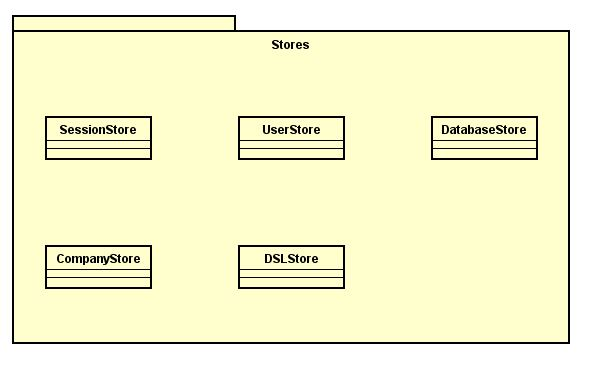
\includegraphics[width=0.8\textwidth]{res/sections/imgs/stores-diagram.jpg}
\caption{Diagramma delle classi per il \glossaryItem{package} Stores}
\end{figure}

\paragraph*{Descrizione del \glossaryItem{package}}
Il \glossaryItem{package} in questione contiene le classi che implementano il concetto di Store presentato nell'architettura Flux. Ciascuno Store contiene dei dati omogenei tra loro e si occupa di fornirli alle pagine che ne necessitano.
\paragraph*{Classi contenute}
\begin{itemize}
\item \textbf{SessionStore};
\item \textbf{UserStore};
\item \textbf{DatabaseStore};
\item \textbf{CompanyStore};
\item \textbf{DSLStore}.
\end{itemize}

\subsubsection{SessionStore}
\paragraph*{Descrizione della classe}
Classe che contiene i dati relativi alla sessione corrente.
\paragraph*{Utilizzo}
Classe che viene utilizzata dall'applicazione per contenere e fornire i dati relativi alla sessione corrente. Si occupa di gestire le \textit{action} relative alla sessione e di conservarne i dati.
\paragraph*{Relazione con altre classi}
\begin{itemize}
\item Router: il router utilizza i dati di SessionStore per identificare quali pagine sono ammesse all'utente.
\item Pages: SessionStore fornisce i dati riferiti alla sessione aperta dall'utente alle pagine.
\end{itemize}

\subsubsection{UserStore}
\paragraph*{Descrizione della classe}
Classe che si occupa di contenere i dati relativi agli User.
\paragraph*{Utilizzo}
Questa classe viene utilizzata per mantenere i dati riguardanti gli utenti e di fornirli alle pagine che li richiedono.
\paragraph*{Relazione con altre classi}
\begin{itemize}
\item Pages: UserStore fornisce i dati riferiti agli utenti alle pagine che devono mostrarli e/o modificarli;
\item Dispatcher: UserStore usa il metodo register di Dispatcher per dichiarare quali \glossaryItem{Action} è in grado di ricevere ed elaborare.
\end{itemize}

\subsubsection{DatabaseStore}
\paragraph*{Descrizione della classe}
Classe che si occupa di contenere i dati relativi alle connessioni ai database definiti per le \glossaryItem{Company}.
\paragraph*{Utilizzo}
Questa classe viene utilizzata per contenere i dati riguardanti le connessioni dei database definiti per le \glossaryItem{Company}. Si occupa di ricevere dal dispatcher le \textit{action} relative a questi dati e di mantenere i dati riferiti.
\paragraph*{Relazione con altre classi}
\begin{itemize}
\item Pages: DatabaseStore fornisce i dati riferiti ai database alle pagine che devono mostrarli e/o modificarli;
\item Dispatcher: DatabaseStore usa il metodo register di Dispatcher per dichiarare quali \glossaryItem{Action} è in grado di ricevere ed elaborare.
\end{itemize}

\subsubsection{CompanyStore}
\paragraph*{Descrizione della classe}
Classe che si occupa di contenere i dati relativi alle \glossaryItem{Company}.
\paragraph*{Utilizzo}
Questa classe viene utilizzata per ricevere le \textit{action} relative alle \glossaryItem{Company} al fine di mantenere i dati relativi ad esse. Inoltre fornisce i metodi per fornire tali dati alle pagine che li richiedono
\paragraph*{Relazione con altre classi}
\begin{itemize}
\item Dispatcher: CompanyStore usa il metodo register di Dispatcher per dichiarare quali \glossaryItem{Action} è in grado di ricevere ed elaborare.
\item Pages: CompanyStore fornisce i dati relativi alla \glossaryItem{Company} alle pagine che possono mostrarli o modificarli.
\end{itemize}

\subsubsection{DSLStore}
\paragraph*{Descrizione della classe}
Classe che si occupa di contenere i dati delle specifiche \glossaryItem{DSL}
\paragraph*{Utilizzo}
Questa classe fornisce i metodi per ricevere le \glossaryItem{Action} relative alle specifiche \glossaryItem{DSL} e per mantenere i dati relativi ad esse. Fornisce inoltre i metodi per disporre quei dati per le pagine che li richiedono.
\paragraph*{Relazione con altre classi}
\begin{itemize}
\item Dispatcher: DSLStore usa il metodo register di Dispatcher per dichiarare quali \glossaryItem{Action} è in grado di ricevere ed elaborare.
\item Pages: DSLStore fornisce i dati relativi alle specifiche \glossaryItem{DSL} alle pagine che possono mostrarli, elaborarli o modificarli.
\end{itemize}


\subsection{Application}
\paragraph*{Descrizione della classe}
Questa è la classe principale del frontend: è la classe che richiama il Router e che inizializza il frontend.
\paragraph*{Utilizzo}
Viene utilizzata per inizializzare il frontend e per fornire le configurazioni necessarie al funzionamento per l'applicazione.

\subsection{Router}
\paragraph*{Descrizione della classe}
Questa classe è necessaria all'applicazione per determinare quale pagina mostrare.
\paragraph*{Utilizzo}
Viene istanziata nell'applicazione principale e determina le associazioni tra pagine e gli indirizzi URL per identificarle.

\subsection{Pages}
\paragraph*{Descrizione del \glossaryItem{package}}
Questo \glossaryItem{package} contiene tutte le pagine richiamate da Router. Ciascuna classe rappresenta una pagina definita come componente React e fornisce i metodi alla pagina per recuperare i dati da mostrare dagli store e i metodi per richiamare gli ActionCreators per la creazione di nuove \glossaryItem{Action}.
